\documentclass[tikz,border=10pt]{standalone}
\usepackage{tikz}
\usetikzlibrary{calc}

\begin{document}
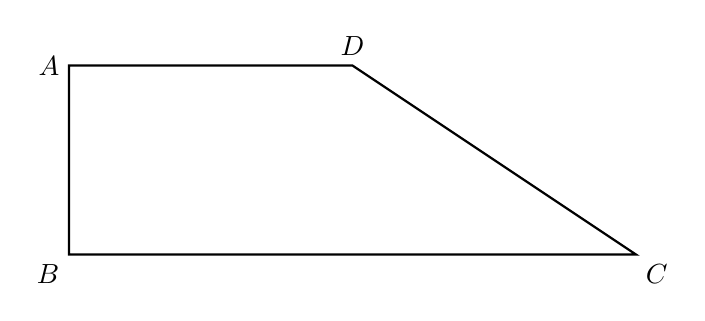
\begin{tikzpicture}[scale=1.2, >=stealth]
    % --- 1. 定义坐标点 ---
    % 设 A 为原点上方点，根据视觉比例设定参数
    \coordinate (A) at (0, 2);
    \coordinate (B) at (0, 0);
    \coordinate (D) at (3, 2);
    \coordinate (C) at (6, 0);

    \draw[thick] (A) -- (B) -- (C) -- (D) -- cycle; % 事实上 A-F-G 是一条线

    % --- 3. 标注文本 ---
    \node[left] at (A) {$A$};
    \node[below left] at (B) {$B$};
    \node[below right] at (C) {$C$};
    \node[above] at (D) {$D$};

\end{tikzpicture}
\end{document}